% Table A.1: its generator renders this table as an image only (no .md/.tex source), so the rendered page(s) are placed
% in a table environment. Copy the PDFs from figures/ alongside (named below).
\begin{table}[p]
\centering
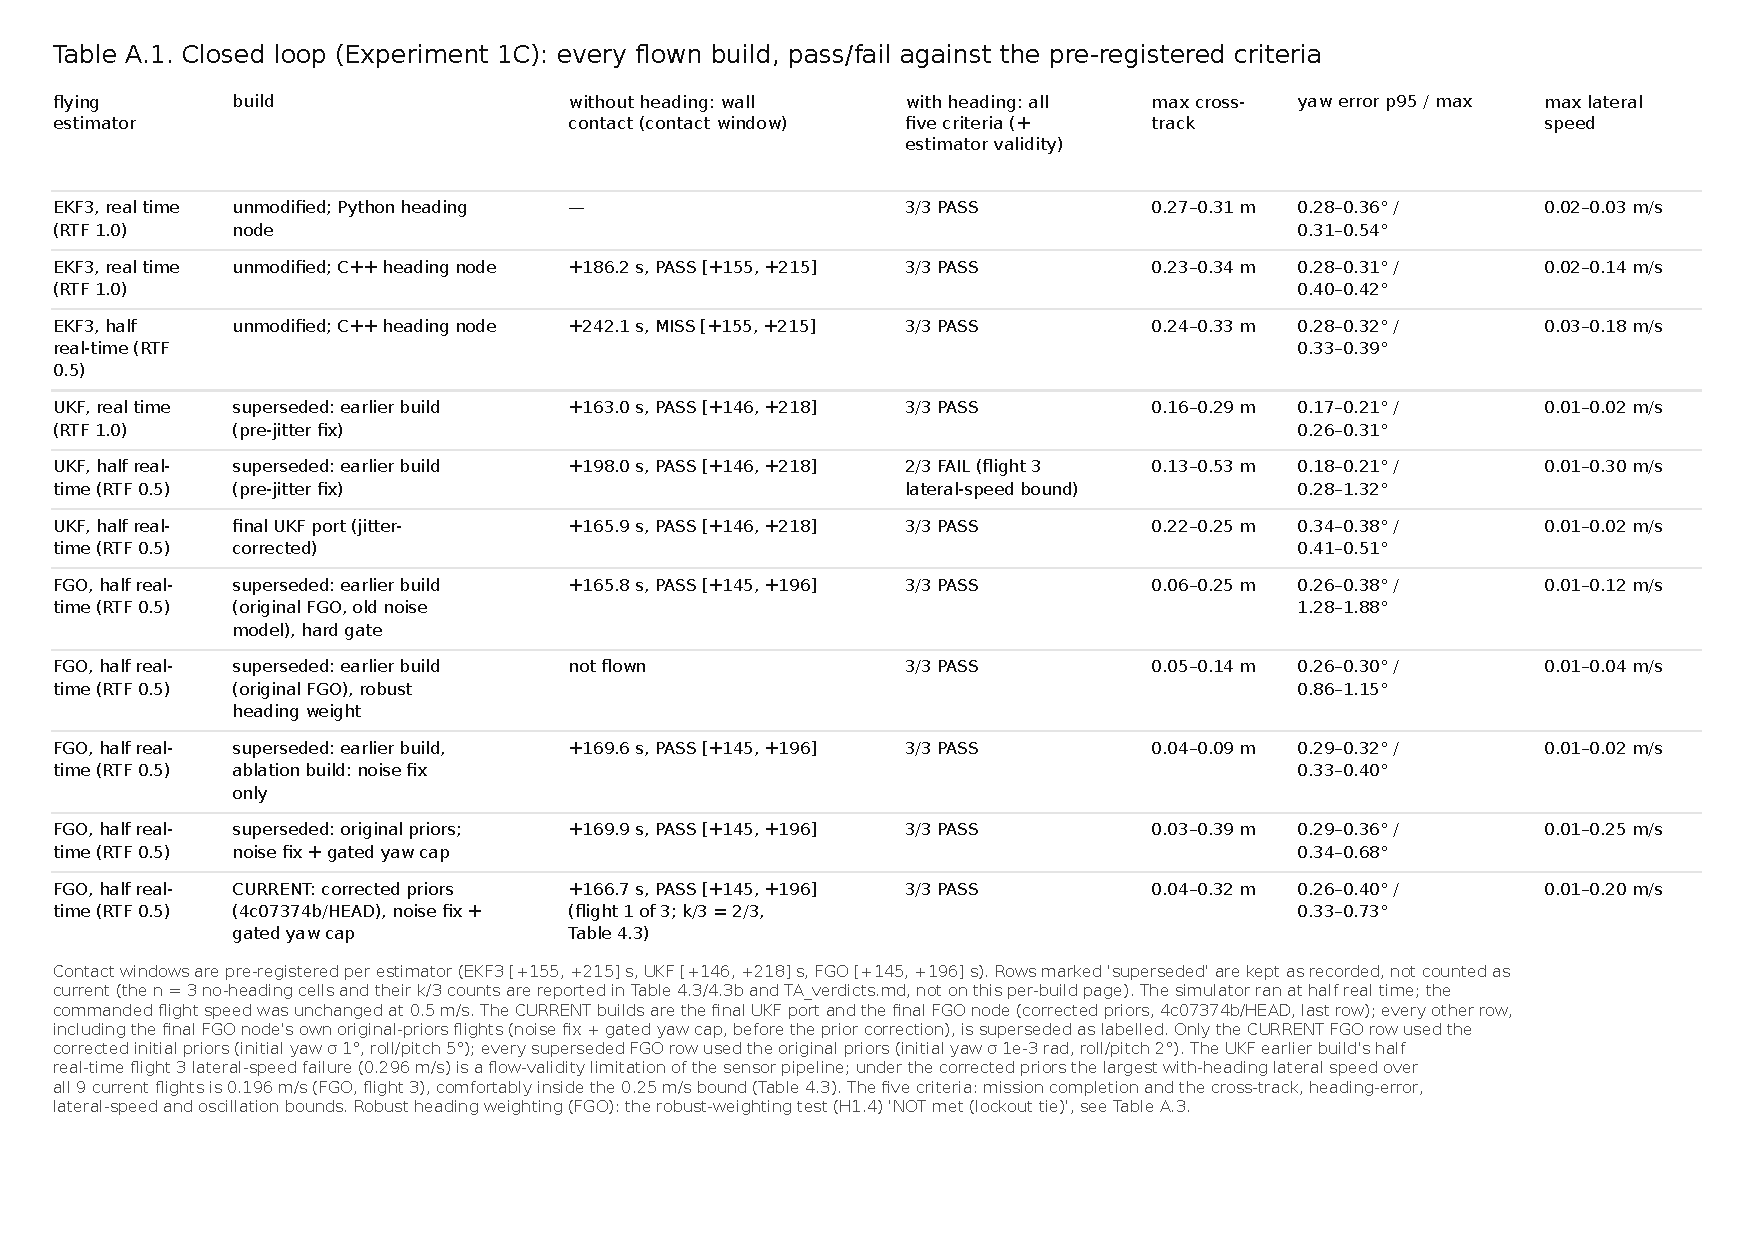
\includegraphics[width=\linewidth]{figures/tab_A-1_p1.pdf}\par\medskip
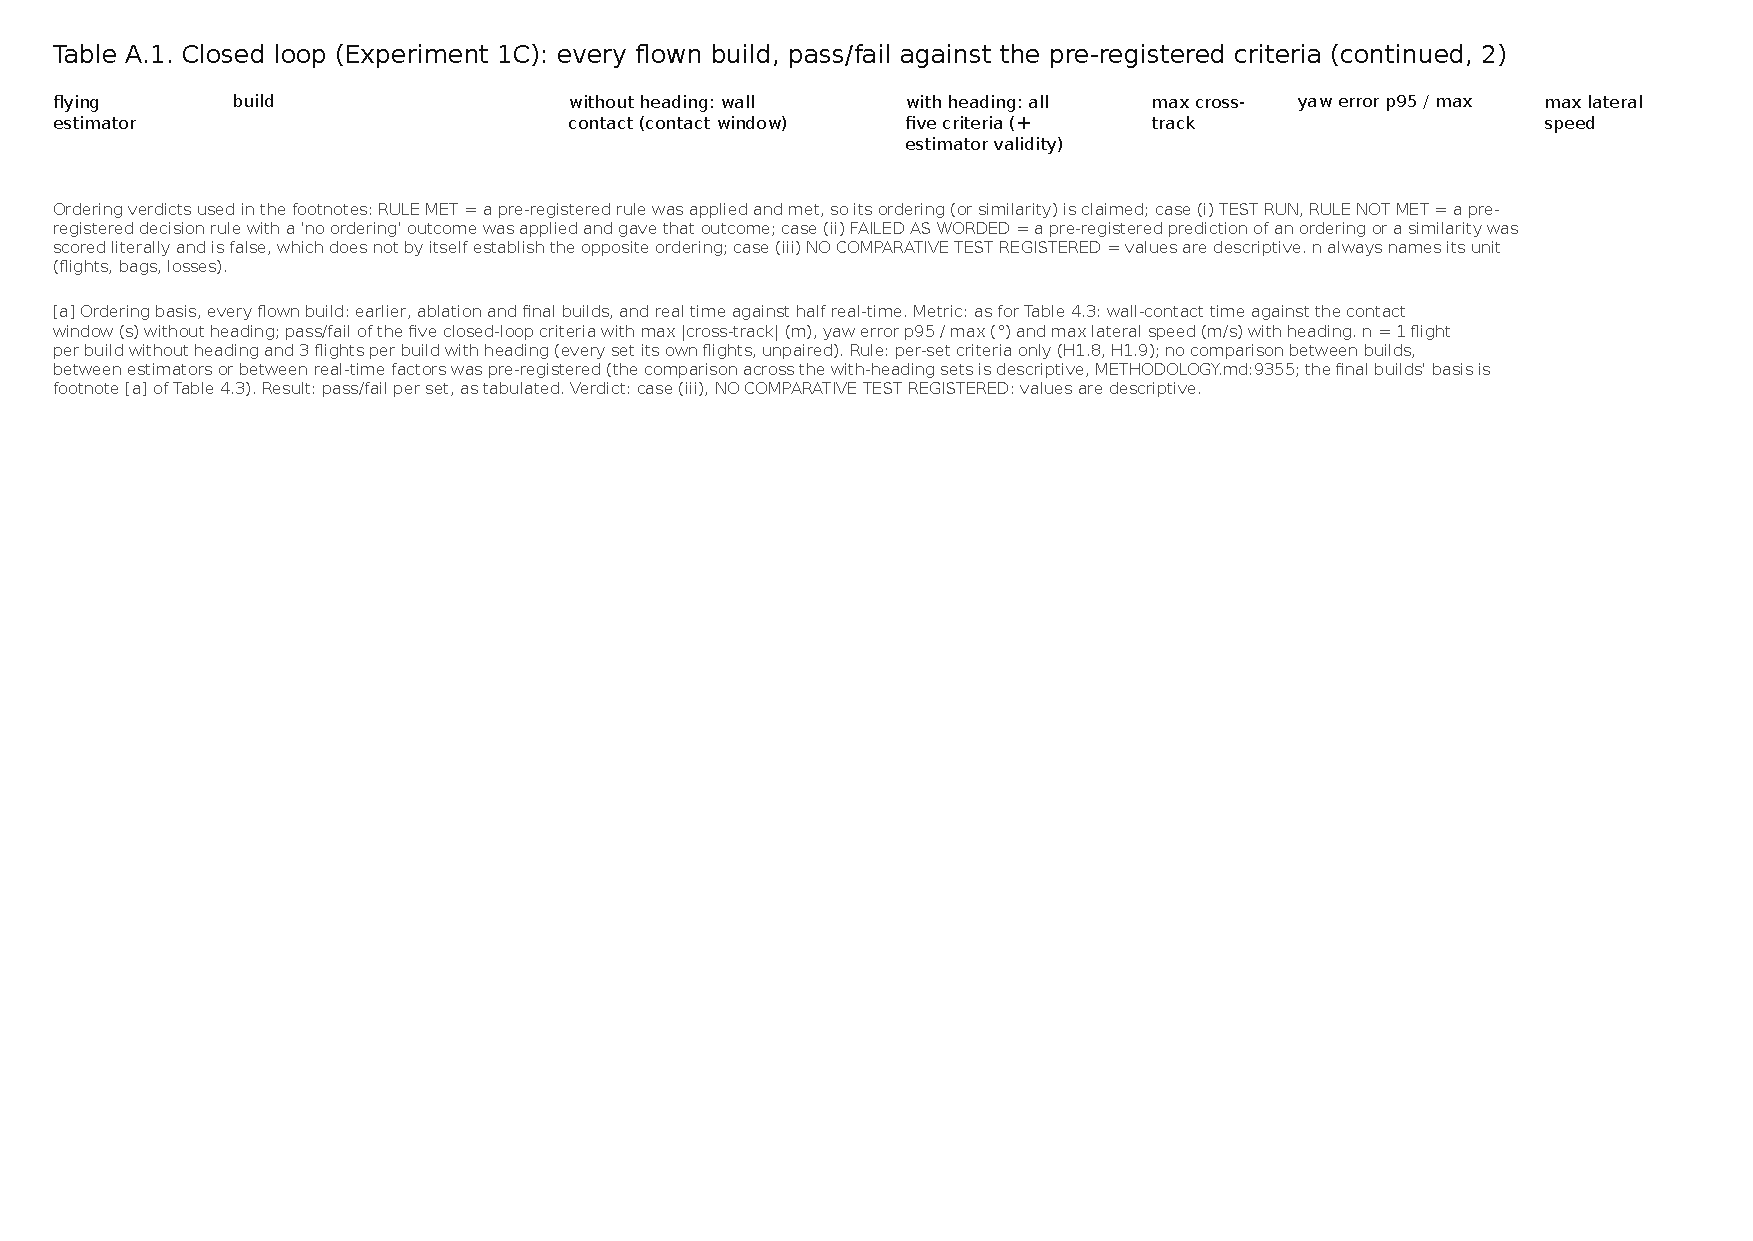
\includegraphics[width=\linewidth]{figures/tab_A-1_p2.pdf}\par\medskip
\caption{Table A.1. Closed loop: every flown build against the five closed-loop criteria and the contact window. Pass/fail of every closed-loop corridor set, computed from the closed-loop score files, with the build ablations labelled: the UKF earlier build (pre-jitter fix, superseded) against the final UKF port (CURRENT); the FGO earlier build (original, hard-gated and robust, superseded), the ablation build (noise fix only, superseded) and the final FGO node, superseded on the original priors and then CURRENT once re-flown on the corrected priors (4c07374b/HEAD, 2026-11-12 regeneration, last row); no ordering between builds or estimators is claimed [a]. Verdict rows: as Figure 4.1/4.1b (H1.8, H1.9, per build; docs/thesis/tables/TA\_verdicts.md).}
\label{tab:A-1}
\end{table}
